\documentclass[conference]{IEEEtran}
\usepackage{amsmath,amssymb,graphicx,booktabs}
\usepackage{pgfplots}
\pgfplotsset{compat=1.18}
\usepackage[hidelinks]{hyperref}
\newcommand{\R}{\mathbb{R}}
\newcommand{\Q}{\mathcal{Q}}
\newcommand{\norm}[1]{\lVert#1\rVert}
\title{Convex Quadratic and Second-Order Cone Constraints in PIQP}
\author{\IEEEauthorblockN{Working draft}}
\begin{document}
\maketitle
\begin{abstract}
We describe an additive C++ extension of PIQP for convex quadratic inequalities and affine second-order cones. A separate primal--dual iteration retains native quadratic objectives and constraints, while reusing PIQP's dense, sparse, and multistage factorizations without changing their interfaces. Symmetric cone whitening converts regularized Nesterov--Todd blocks into scalar dual blocks. A spectral representation applies this transformation in linear time and avoids dense cone scaling matrices. We derive the mixed Newton system, quadratic corrector terms, and finite-precision recovery rules. Numerical tests check independently constructed optimality conditions and allocation-free solves and updates. Experiments compare native and conic representations, multistage horizon scaling, and public conic problems on an Apple Silicon laptop. The method is a practical extension; no general convergence or infeasibility-certificate claim is made.
\end{abstract}

\section{Introduction}
Quadratic constraints occur in terminal sets, energy limits, and ellipsoidal regions in optimal control. Second-order cones also express norm limits and contact friction. Approximating these constraints with affine inequalities can increase model size or introduce conservatism. A solver that handles them directly can retain the original convex model.

PIQP combines a primal--dual interior-point iteration with proximal regularization and specialized linear algebra~\cite{piqp}. Its multistage backend detects and factors block tridiagonal matrices with a dense border~\cite{multistage}. Native quadratic constraints have a direct precedent in HPIPM~\cite{hpipm}. ECOS~\cite{ecos}, QOCO~\cite{qoco}, and Clarabel~\cite{clarabel} provide complementary examples of conic scaling, regularization, and sparse implementation.

This work asks how much of the existing PIQP implementation can be reused for mixed quadratic and conic constraints. The extension changes neither the QP iteration nor the backend interface. Its main numerical device is a regularized symmetric whitening transformation, evaluated without forming a dense cone block. The resulting Newton data can pass through every existing factorization. Whole-constraint sparsity, original-coordinate stopping tests, and finite-precision recovery require separate treatment.

\section{Problem and proximal Newton system}
Consider
\begin{subequations}\label{eq:model}
\begin{align}
 \min_x\quad &\tfrac12x^TPx+c^Tx,\\
 \text{subject to}\quad &Ax=b,\\
 &g_i(x)=\tfrac12x^TQ_ix+q_i^Tx-u_i\leq0,\\
 &F_jx+f_j\in\Q^{d_j},
\end{align}
\end{subequations}
where $P,Q_i\succeq0$ and $\Q^d=\{(t,v):t\geq\norm{v}_2\}$. Affine inequalities and bounds are scalar constraints with zero curvature. Local index sets restrict a constraint to selected components of $x$. Rotated cones use the transformation
\begin{equation}
 T(a,b,v)=(a+b,a-b,\sqrt2v).
\end{equation}
If $s_o,z_o$ are ordinary-cone variables, the corresponding rotated variables are $s_r=T^{-1}s_o$ and $z_r=T^Tz_o$. The different transformations preserve $z_o^TTs_r$.

Stack the scalar functions and cone rows $-F_jx-f_j$ in $g(x)$. With independent slacks $s$ and duals $z$ in the product cone, write $g(x)+s=0$. Let
\begin{equation}
 J=g'(x),\qquad H=P+\sum_i z_iQ_i.
\end{equation}
The unregularized Karush--Kuhn--Tucker (KKT) residuals are
\begin{equation}
 r_d=Px+c+A^Ty+J^Tz,\quad r_e=Ax-b,\quad r_g=g(x)+s.
\end{equation}
For centers $(\xi,\eta,\zeta)$ and positive $\rho,\delta$, use
\begin{equation}\label{eq:prox}
 \bar r_d=r_d+\rho(x-\xi),\quad
 \bar r_e=r_e-\delta(y-\eta),\quad
 \bar r_g=r_g-\delta(z-\zeta).
\end{equation}
The objective matrix $P$ remains separate from $H$ in storage and objective evaluation.

\subsection{Scaling and elimination}
For a Lorentz cone the Jordan product is
\begin{equation}
 (a,u)\circ(b,v)=(ab+u^Tv,av+bu),\qquad e=(1,0).
\end{equation}
We use the barrier $-\tfrac12\log(a^2-\norm{u}_2^2)$ and count one complementarity degree per cone and per scalar inequality~\cite{cvxopt}. Thus $\mu=s^Tz/\nu$, where $\nu$ is this number of blocks, not their total coordinate dimension.

Let $W=W^T\succ0$ be the Nesterov--Todd scaling with $\lambda=Wz=W^{-1}s$. Define $L_\lambda v=\lambda\circ v$. A scaled complementarity right-hand side $r_c$ gives
\begin{equation}
 W^{-1}\Delta s+W\Delta z=h,\qquad h=L_\lambda^{-1}r_c.
\end{equation}
Eliminating slack yields
\begin{equation}\label{eq:newton}
 \begin{bmatrix}H+\rho I&A^T&J^T\\A&-\delta I&0\\J&0&-D\end{bmatrix}
 \begin{bmatrix}\Delta x\\\Delta y\\\Delta z\end{bmatrix}
 =\begin{bmatrix}-\bar r_d\\-\bar r_e\\-\bar r_g-Wh\end{bmatrix}.
\end{equation}
Here $D=W^2+\delta I$. For scalar constraints $D=s/z+\delta$. For cones it is positive definite. Eliminating the regularized dual variables produces
\begin{equation}\label{eq:condensed}
 H+\rho I+\delta^{-1}A^TA+J^TD^{-1}J\succ0.
\end{equation}
This explains compatibility with PIQP's factorizations in exact arithmetic. It does not establish convergence of the nonlinear iteration.

\subsection{Predictor and corrector}
The affine predictor uses $h_a=-\lambda$. From its admissible step, compute $\mu_a$ and set $\sigma=(\min\{1,\max\{0,\mu_a/\mu\}\})^3$. For a combined corrector use
\begin{equation}\label{eq:corrector}
 h=-\lambda+L_\lambda^{-1}\left(\sigma\mu e
 -(W^{-1}\Delta s_a)\circ(W\Delta z_a)\right).
\end{equation}
Writing the predictor contribution explicitly avoids dividing the difference of nearly equal Jordan products.

Native quadratic constraints have exact second-order residual terms
\begin{equation}
 \tfrac12\Delta x_a^TQ_i\Delta x_a,\qquad
 \sum_i\Delta z_{a,i}Q_i\Delta x_a.
\end{equation}
Subtract these from the feasibility and stationarity right-hand sides, respectively. One common primal and dual step preserves these factors. A fraction-to-boundary rule keeps independent slacks and duals interior.

Backtracking evaluates the actual nonlinear residuals in~\eqref{eq:prox}, with centers, target $\sigma\mu$, and scaling $W$ fixed. The complementarity merit uses $(W^{-1}s)\circ(Wz)-\sigma\mu e$. A rejected combined direction is replaced by a centered direction without predictor remainders. Centers move when the corresponding original residual decreases. Regularization decreases with complementarity; a failed factorization or inaccurate affine-predictor solve triggers increased regularization and another solve. These are practical safeguards, rather than conditions of a proved convergence theorem.

\section{Numerical implementation}
\subsection{Linear-time cone whitening}
Set $B=(W^2+\delta I)^{-1/2}$. The substitutions
\begin{equation}\label{eq:white}
 \widetilde J=BJ,\quad v=B^{-1}\Delta z,\quad
 \widetilde r_g=-B\bar r_g-BWh
\end{equation}
replace each cone dual block by $-I$. Recover $\Delta z=Bv$. The existing backend therefore receives only scalar dual scaling, with transformed Jacobian rows and right-hand sides.

A Lorentz scaling has the form
\begin{equation}
 W=\beta\begin{bmatrix}w_0&w_v^T\\w_v&I+w_vw_v^T/(1+w_0)\end{bmatrix},
 \quad w_0^2-\norm{w_v}_2^2=1.
\end{equation}
Let $r=\norm{w_v}_2$. If $r=0$, then $W=\beta I$. Otherwise set $u=w_v/r$. In the span of the leading axis and $(0,u)$, the eigenvalues are $\beta(w_0+r)$ and $\beta/(w_0+r)$. On the orthogonal complement the eigenvalue is $\beta$. Applying $W$, $W^{-1}$, $B$, or $BW$ therefore requires one tail inner product and a vector update. Storage and arithmetic are $O(d)$ per application. Rationalized coefficients avoid subtraction of nearly equal eigenvalues for small $r$.

The order in~\eqref{eq:white} matters. The eigenvalues of $BW$ are $\omega/\sqrt{\omega^2+\delta}\leq1$. Applying this bounded product directly avoids first creating the potentially ill-conditioned vector $Wh$. Likewise, recover cone slack steps from the original affine feasibility equation,
\begin{equation}\label{eq:recovery}
 \Delta s=-\bar r_g-J\Delta x+\delta\Delta z,
\end{equation}
instead of subtracting $W^2\Delta z$ from $Wh$. Independent near-boundary Newton tests check both feasibility and scaled complementarity.

\subsection{Sparse and multistage structure}
A cone's transformed rows can depend on the union of all columns touched by that cone. Setup allocates this union, including stored zeros. A quadratic block reserves its Hessian pattern and every possible Jacobian entry. Numerical updates never infer support from current values, which could vanish at the initial iterate.

The implementation retains sparse objective and equality matrices and small local constraint blocks. Dense Cholesky, sparse LDL$^T$, and the existing BLASFEO multistage factorization consume the same transformed equations. When each entire constraint is confined to neighboring stages and a bounded global-variable border,~\eqref{eq:condensed} retains the multistage structure. With bounded local dimensions and constraint work per stage, assembly and factorization have linear horizon complexity per iteration. A horizon-wide energy constraint or a cone joining distant stages can destroy this property.

Whitening avoids dense $d\times d$ scaling matrices, but it can still fill a sparse cone's transformed rows. Its work is $O(dk)$ for support size $k$. The experiments separate cone dimension from support size to expose this cost. No alternative sparse expansion is assumed to be faster without measurement.

\subsection{Scaling, initialization, and termination}
Diagonal variable scaling $x=E\hat x$ and a positive objective multiplier $\gamma$ give $\hat P=\gamma E^TPE$. A scalar constraint multiplier $\alpha_i$ scales its entire quadratic expression, including $\hat Q_i=\alpha_iE^TQ_iE$. Each cone receives a common row multiplier $\beta_j$. Independent row scaling within a cone is not valid. Scale selection includes curvature, even when the current quadratic gradient is zero.

An auxiliary regularized solve initializes the objective, affine constraints, and cones with unit slack scaling. Quadratic rows are excluded from that auxiliary model, then evaluated at its primal point. Scalar pairs are made positive, and cone pairs are shifted along their leading axis. Each solve starts from scratch while reusing symbolic factorizations and allocated memory.

Return quadratic and cone slacks divided by their constraint scales and duals multiplied by their constraint scales divided by $\gamma$. Stopping evaluates the original model, including true quadratic values, cone membership, slack consistency, stationarity, and complementarity. The reported complementarity is not described as an unconditional objective gap. For singular Lagrangian Hessians, an exact dual objective would also require a range condition. Unresolved cases return an iteration limit or numerical failure, not an inferred conic infeasibility certificate.

\section{Experiments}
\subsection{Protocol and validation}
Experiments use an Apple M4 Max MacBook with 48\,GiB unified memory, macOS 26.6.2, Apple Clang 21.0.0, Eigen 5.0.1, and an installed BLASFEO archive targeting Apple M1 instructions. The release build uses \texttt{-O3 -DNDEBUG} and double precision. Clarabel 0.11.1 runs through Python 3.13 with NumPy 2.2.6 and SciPy 1.15.3. Solver threads are limited to one. Benchmark processes run sequentially, without concurrent builds or tests. Normal operating-system scheduling remains active, with no core pinning, frequency lock, or temperature control. Consequently these are laptop measurements, not controlled hardware throughput estimates.

The generated suite has 18 deterministic instances: diagonal ellipsoids at three dimensions in native and rotated-cone form, three locally coupled mixed problems, four double-integrator control horizons, and five cone dimensions at fixed two-variable support. The control model has four states, two inputs, 0.2\,s sampling, acceleration norm at most one, and a terminal state ball of radius 0.5. Two continuous plastic-plate problems from CBLIB~\cite{cblib}, \texttt{nql30} and \texttt{nql60}, add 4,501 and 18,001 variables, respectively. They have 3,680 and 14,560 equalities and 900 and 3,600 cones. Both use the general sparse backend.

Each timing batch follows one unrecorded solve. Generated PIQP batches and all Clarabel batches contain 30 solves, while public PIQP batches contain ten. Every solve initializes from scratch. Setup is measured once per instance and backend. Update timings reapply unchanged quadratic bounds and cone offsets. Clarabel timings include the Python call but exclude conversion to the conic model. Table~\ref{tab:time} reports medians, and the archived CSV files retain every observation, residual, status, and the first and third quartiles. Repetitions measure timing dispersion, not additional problem instances.

PIQP requests absolute and relative tolerances of $10^{-8}$. Clarabel requests $10^{-11}$, since looser internal criteria on the plate problems did not meet the same original-coordinate complementarity check. Independent acceptance requires primal feasibility, stationarity, dual-cone membership, and slack consistency within $10^{-7}$, finite variables, and $s^Tz/(1+|f(x)|)\leq10^{-7}$. A rounding allowance applies to nonnegativity of $s^Tz$. Generated PIQP solutions also agree across backends and with available analytic solutions within $10^{-4}$ in maximum norm.

All 54 generated instance/backend combinations and both public solves pass these checks. Clarabel passes its conic-form checks on all 20 instances, with seven \texttt{Solved} and 13 \texttt{AlmostSolved} statuses. However, mapping the lifted duals back to native quadratic multipliers leaves stationarity above $10^{-7}$ on the three native ellipsoid and three mixed instances. Their recovered residuals range from $1.35\times10^{-7}$ to $2.38\times10^{-6}$. These timings therefore do not establish an advantage at matched native-dual accuracy. The supplied conic ellipsoids do pass the conic checks. Across all instances, objective differences remain below $6\times10^{-8}$.

The C++ suite adds 45 tests, including 50 mixed problems with independently constructed KKT points, full Newton-direction comparisons, singular curvature, zero gradients, cone apexes, scale variation, nearly dependent equalities, nonlocal support, and known infeasible models. Tests exercise every sparse elimination mode and the actual BLASFEO multistage factorization. Eigen allocation guards and a C++ allocation counter cover solves and numerical updates. The extension passes AddressSanitizer and UndefinedBehaviorSanitizer checks. Existing QP tests also pass. Infeasible tests check that the solver does not claim a successful solution, rather than demand a certificate that this method does not derive.

\begin{table}[t]
\centering
\caption{Median solve time in milliseconds. Clarabel uses exact cone reformulations for native quadratic rows.}
\label{tab:time}
\small\begin{tabular}{lrrrr}
\toprule
Instance & Dense & Sparse & Multi. & Clarabel\\
\midrule
Quadratic, $n=128$ & 0.630 & 0.050 & 0.255 & 0.216\\
Cone lift, $n=128$ & 1.032 & 8.082 & 1.383 & 0.232\\
Mixed, 64 stages & 4.317 & 0.525 & 0.763 & 1.632\\
Control, $N=80$ & 21.337 & 0.661 & 0.733 & 0.986\\
nql30 & -- & 85.242 & -- & 98.662\\
nql60 & -- & 490.676 & -- & 620.653\\
\bottomrule
\end{tabular}

\end{table}

\begin{figure*}[t]
\centering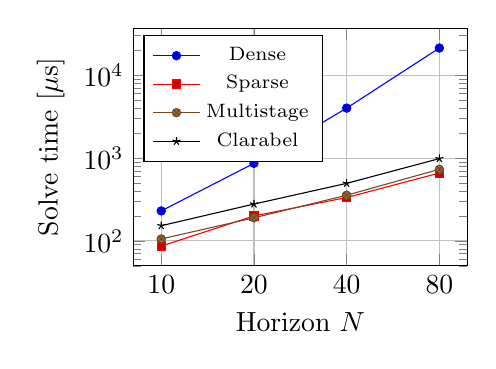
\begin{tikzpicture}
\begin{loglogaxis}[width=.48\textwidth,height=4.6cm,xlabel={Horizon $N$},ylabel={Solve time [$\mu$s]},grid=major,xtick={10,20,40,80},xticklabels={10,20,40,80},legend style={font=\scriptsize},legend pos=north west]
\addplot+[mark size=1.5pt] coordinates {(10,230.354) (20,864.646) (40,4016.31) (80,21337.3)};
\addlegendentry{Dense}
\addplot+[mark size=1.5pt] coordinates {(10,86.625) (20,200.166) (40,334.375) (80,660.604)};
\addlegendentry{Sparse}
\addplot+[mark size=1.5pt] coordinates {(10,105.645) (20,190.041) (40,356.333) (80,732.875)};
\addlegendentry{Multistage}
\addplot+[mark size=1.5pt] coordinates {(10,152.625) (20,278.771) (40,495.646) (80,986.208)};
\addlegendentry{Clarabel}
\end{loglogaxis}
\end{tikzpicture}
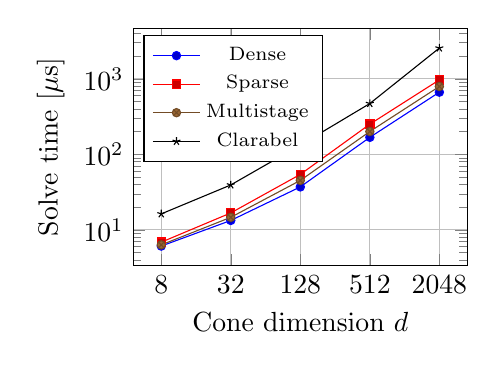
\begin{tikzpicture}
\begin{loglogaxis}[width=.48\textwidth,height=4.6cm,xlabel={Cone dimension $d$},ylabel={Solve time [$\mu$s]},grid=major,xtick={8,32,128,512,2048},xticklabels={8,32,128,512,2048},legend style={font=\scriptsize},legend pos=north west]
\addplot+[mark size=1.5pt] coordinates {(8,6.1045) (32,13.333) (128,37.0625) (512,167.896) (2048,664.98)};
\addlegendentry{Dense}
\addplot+[mark size=1.5pt] coordinates {(8,6.875) (32,16.7705) (128,54.2495) (512,250.75) (2048,967.375)};
\addlegendentry{Sparse}
\addplot+[mark size=1.5pt] coordinates {(8,6.334) (32,14.667) (128,45.1665) (512,200.5) (2048,791.729)};
\addlegendentry{Multistage}
\addplot+[mark size=1.5pt] coordinates {(8,16.291) (32,39.333) (128,132.562) (512,470.604) (2048,2553.94)};
\addlegendentry{Clarabel}
\end{loglogaxis}
\end{tikzpicture}

\caption{Median solve times. Left: control horizon with fixed stage dimensions. Right: cone dimension with fixed two-variable support. The right experiment isolates coordinate work and does not represent a cone with growing variable support.}
\label{fig:scaling}
\end{figure*}

\subsection{Structure and representation}
Figure~\ref{fig:scaling} shows nearly linear control-horizon growth for both sparse and multistage solves. Both take seven iterations at every horizon. The measurements show no consistent multistage speed advantage for these small stage blocks. Dense factorization grows much faster with the horizon. At fixed support, the cone sweep is also approximately linear after the smallest sizes, as expected from the spectral transforms. Iteration counts rise from five to seven over that sweep.

The $n=128$ ellipsoid exposes a different limitation. A native scalar quadratic row retains a small augmented sparse system. Its exact cone lift expands the slack dimension and fills the transformed Jacobian across the entire variable support. The sparse cone solve is much slower than both the native solve and Clarabel on the identical conic representation. Linear-time scaling alone does not remove this fill. A sparse expansion of the cone block, as used by ECOS, is not implemented here. The native quadratic representation avoids that particular expansion cost, but general large-support cones remain a weakness of the whitening adapter.

\subsection{Public problems and profile}
Both plate solutions agree with Clarabel in objective within $7\times10^{-9}$. Their PIQP stationarity residuals are $2.34\times10^{-9}$ and $1.57\times10^{-9}$, and primal violations are below $4\times10^{-14}$. The solve-time interquartile ranges are 84.7--86.2\,ms and 484.9--500.5\,ms. They require 22 and 21 iterations, with 26 and 29 regularization retries and 106 and 95 refinement steps. The retry counts explain why iteration count alone understates their linear-algebra work.

A separate Tracy 0.12.2 capture of 20 \texttt{nql30} solves attributes 38.5\% of exclusive recorded time to sparse numerical factorization and 32.3\% to triangular solves. Newton assembly accounts for 6.9\%. These instrumented timings diagnose cost and are excluded from Table~\ref{tab:time}. Earlier dense cone-scaling matrices were replaced by the spectral operations in Section III-A. This removes cubic cone factorization and quadratic cone storage. Two subsequent experiments used three samples per public problem and variant. Delaying regularization reduction for two iterations after retries, or retaining the raised value as a floor, reduced median solve times by approximately 21--27\%. Neither change was adopted because its difficult-case validation was too narrow.

The transformed Jacobians contain 8,100 and 32,400 stored entries. The permuted upper KKT matrices contain 36,850 and 147,500 entries, while their factors contain 122,642 and 610,684 entries including the diagonal. These symbolic counts include declared numerical zeros but exclude index arrays and other workspaces. Separate process peak resident sizes are 15.8 and 49.5\,MiB. Those observations include input loading, model copies, symbolic counting, and libraries, rather than just solver workspaces. Setup, update, and factorization-plus-assembly timings are retained with the raw data.

The QP regression compares identical box-constrained problems against the original revision, using the same compiler and $10^{-10}$ tolerances. Both versions pass the analytic solution check. The QP implementation is unchanged. Laptop timing variability prevents conclusions about small overhead differences.


\newpage
\section{Conclusion}
The extension reuses PIQP's factorization implementations for mixed convex quadratic and Lorentz constraints. Its additional numerical work lies in nonlinear residuals and curvature, scaled complementarity, structure-preserving assembly, and accurate recovery. The measurements characterize this implementation on the tested problems; they do not establish a general performance ordering or convergence theorem.

\bibliographystyle{IEEEtran}
\bibliography{references}
\end{document}
